\section{Representative Examples}

Given the theoretical framework for downfolding a many-orbital (or many electron) problem to a 
few orbital (or few electron) problem, we now discuss few examples which also serve to highlight some practical aspects 
associated with AIDMD. The first example is mostly pedagogical, 
where we have completely avoided the \textit{ab-initio} related complications of AIDMD. Rather, we use information directly available 
from \textit{exact} eigenstates themselves to downfold from a lattice model with more orbitals (3-band model) 
to one with fewer orbitals (1-band model). We then gradually increase the complexity of the problems we address 
by downfolding the hydrogen chain in one dimension (with up to 10 atoms) and graphene 
(with up to 32 carbons on a 2D honeycomb lattice). Finally, we use the matching pursuit algorithm discussed 
in section 2, suited for multiple energy scales, for the case of transition metals 
by considering the diatomic FeSe molecule.

\lucas{What about this? } 
The examples are as follows:
\begin{itemize}
\item Section~\ref{subsection:3band}: Three band Hubbard $\rightarrow$ one band Hubbard at half filling. Demonstrates finding a basis set for the second quantized operators and uses a set of eigenstates directly sampled from the low-energy space to find a one-band model.
\item Section~\ref{subsection:1dhydrogen}: Hydrogen chain $\rightarrow$ one band Hubbard model at half filling. Demonstrates basis sets for {\it ab-initio} systems and the possibility to use this technique to determine the quality of a model to a given physical situation.
\item Section~\ref{subsection:graphene}: Graphene $\rightarrow$ one band Hubbard model with and without $\sigma$ electrons. Demonstrates using the downfolding procedure to examine the effects of screening due to core electrons. 
\item Section~\ref{subsection:fese}: FeSe molecule $\rightarrow$ $d,p,4s$ system. Demonstrates the use of matching pursuit to assess the importance of terms in an effective model and to select compact effective models.
\end{itemize}



\HJC{Lucas, Is this better?} \lucas{It still looks to me that this really goes in the 3-band part?} 
In all examples we will highlight the important ingredients associated with AIDMD. First and foremost, is the choice 
of low energy space or energy window i.e. how our database of wavefunctions was generated. Associated with this is 
the choice of the one body space in terms of which the effective Hamiltonian is expressed. Finally, we discuss 
aspects of the functional forms or parameterizations that are expected to describe our physical 
problem. In three out of our four representative examples we work with the single (or 1-) band Hubbard Hamiltonian,
\begin{equation}
	\tilde{H} = -t \;\sum_{\langle i,j \rangle} \tilde{d}_i^{\dagger} \tilde{d}_j + U \;\sum_{i} \tilde{n}^{i}_{\uparrow} \tilde{n}^{i}_{\downarrow}
\label{eq:oneband}
\end{equation}
where $t$ and $U$ correspond to downfolded (renormalized) parameters and $\tilde{d}$ are the effective one-particle operators, 
which are obtained from transformations on their bare counterparts. Thus 
the determination of effective Hamiltonians is a \emph{dual} problem - what are the composite objects ($\tilde{d}_i$ here) 
that give a compact description of the low energy physics? and given this choice what 
are the effective interactions between them?

\subsection{Three-band Hubbard model to one band Hubbard model at half filling}
\label{subsection:3band} 
\HJC{Still editing - need to incorporate Lucas suggestions and new results for 8 site FCI}
Our first example is motivated by the high $T_c$ superconducting cuprates~\cite{Bednorz1986} that 
have parent Mott insulators with rich phase diagrams on electron or hole doping~\cite{Dagotto_RevModPhys, LeeWen_RevModPhys}. 
Many works have been devoted to their model Hamiltonians and corresponding parameter 
values~\cite{Emery, ZhangRice, tJSpalek, Hybertsen_PRB1989, Hybertsen_PRB1990, Pavirini, Kent_Hubbard}. 
The emergent consensus of the minimal model involving the oxygens is the 3-orbital or 3-band Hubbard model, 
\begin{eqnarray}
H &=&    \epsilon_p \sum_{j,\sigma} n^{p}_{j,\sigma} + \epsilon_{d} \sum_{i,\sigma}  n^{d}_{i,\sigma} 
	+ t_{pd} \sum_{\langle i,j \rangle, \sigma} \text{sgn}(p_i,d_j) \Big( d_{i,\sigma}^{\dagger} p_{j,\sigma} + \text{h.c.} \Big) \nonumber \\
  & &   + U_p \sum_{j} n^{p}_{j,\uparrow} n^{p}_{j,\downarrow} + U_d \sum_{i} n^{d}_{i,\uparrow} n^{d}_{i,\downarrow} + V_{pd} \sum_{\langle i,j \rangle} n^{j}_p n^{i}_d 
\end{eqnarray}
%\begin{eqnarray}
%H &=&    \epsilon_p \sum_{j,\sigma} n^{p}_{j,\sigma} + \epsilon_{d} \sum_{i,\sigma}  n^{d}_{i,\sigma} 
%	+ t_{pd} \sum_{\langle i,j \rangle, \sigma} \text{sgn}(p_i,d_j) \Big( d_{i,\sigma}^{\dagger} p_{j,\sigma} + \text{h.c.} \Big) + U_p \sum_{j} n^{p}_{j,\uparrow} n^{p}_{j,\downarrow} + U_d \sum_{i} n^{d}_{i,\uparrow} n^{d}_{i,\downarrow} + V_{pd} \sum_{\langle i,j \rangle} n^{j}_p n^{i}_d 
%\end{eqnarray}
where $d_i,p_j$ refer to the  $d_{x^2 - y^2}$ orbitals of copper (at site $i$) and $p_x$ or $p_y$ 
oxygen (at site $j$)  respectively and the signs of the hopping $t_{pd}$ between them are shown in Fig.~\ref{fig:threeband}. 
$\epsilon_d$,$\epsilon_p$ refer to the orbital energies, 
$U_d$, $U_p$ refer to strength of onsite Hubbard interactions and $V_{pd}$ refers to the 
strength of the density-density interactions between a neighboring $p$ and $d$ orbital. 
We keep the exposition simple and consider only the case where $\epsilon_p$, $t_{pd}$ (chosen to be $1.3$ eV throughout) 
and $U_{d}$ are non zero. Since we work with fixed number of particles we set $\epsilon_d = 0$, thus the 
charge transfer energy $\Delta \equiv \epsilon_p - \epsilon_d$ equals $\epsilon_p$ in our notation. 
We work in the hole notation; half filling corresponds to 2$\uparrow$ and 2$\downarrow$ holes on the $2\times2$ cell.
\begin{figure}[htpb]
\centering

\includegraphics[width=0.8\linewidth]{./Figures/three_band_figure.eps}
\caption{Schematic for downfolding the three band Hubbard model to the one band Hubbard model. 
The oxygen orbitals are completely eliminated to give "dressed" $d$-like orbitals of the one band model, with modified hopping 
and interaction parameters.}
\label{fig:threeband} 
\end{figure}	

It is our objective to determine what 1-band parameters best describe the 3-band data, the former defined 
in terms of effective \textit{d-like} orbitals, $\tilde{d}$, which are mixtures of copper and oxygen orbitals; 
this optimal transformation also remains an unknown. We encode the relationship between the 
bare and effective operators as a linear transformation ${\bf T}$, 
\begin{equation}
	\tilde{d}_{i,\sigma} = \sum_{j} T_{ij} c_{j,\sigma}
\end{equation}
where $c_{j,\sigma}$ is the bare hole (destruction) operator and refers to either the bare $d$ or $p$ orbitals. 
Higher body generalizations are also possible, but have not been considered here. 
Accounting for all symmetries of the $2\times2$ unit cell, {\bf T} is a $4 \times 12 $ matrix, with 
the numbering of the orbitals corresponds to Fig.~\ref{fig:threeband}, explicitly written out as, 
\begin{eqnarray}
{\bf T} = 
\left(
\begin{array}{cccccccccccc}
F        & \alpha_2 &        \alpha_2 &  \alpha_4 & \alpha_1 & \alpha_1 & -\alpha_1 & -\alpha_1 & \alpha_3 & -\alpha_3 & \alpha_3 & -\alpha_3 \\
\alpha_2 &  F       &        \alpha_4 &  \alpha_2 & \alpha_3 & -\alpha_1 & \alpha_1 & -\alpha_3 & -\alpha_3 & \alpha_3 & \alpha_1 & -\alpha_1 \\
\alpha_2 & \alpha_4 & F               &  \alpha_2 & -\alpha_1 & \alpha_3 & -\alpha_3 & \alpha_1 & \alpha_1 & -\alpha_1 & -\alpha_3 & \alpha_3 \\
\alpha_4 & \alpha_2 & \alpha_2        &   F       & -\alpha_3 & -\alpha_3 & \alpha_3 & \alpha_3 & -\alpha_1 & \alpha_1 & -\alpha_1 & \alpha_1 \\
\end{array}
\right)
\end{eqnarray}
where we have defined $F \equiv \sqrt{1-4{\alpha_1}^2 - 2{\alpha_2}^2 - 4 {\alpha_3}^2 -{\alpha_4}^2}$ and 
where the parameters $\alpha_1$,$\alpha_2$,$\alpha_3$ and $\alpha_4$ will be optimized to minimize a 
certain cost function, which will be explained shortly. 

The one particle density matrix calculated in eigenstate $s$ in the transformed basis is related to that in the original basis by,
\begin{equation}
	\langle {\tilde{d}_{i,\sigma}}^{\dagger} \tilde{d}_{j,\sigma} \rangle_{s} = \sum_{mn} T^{*}_{im} \langle {c_{m,\sigma}}^{\dagger} c_{n,\sigma} \rangle_{s} T_{jn}
\end{equation}
Using this relationship, we demand two conditions be satisfied, (1) the effective orbitals ($\tilde{d}_{i,\sigma}$) 
are orthogonal to each other and (2) the sum of all diagonal entries of the 1-RDM of the effective orbitals for all low energy eigenstates 
$\sum_{i} \langle {\tilde{d}_{i,\sigma}}^{\dagger} \tilde{d}_{i,\sigma} \rangle_{s}$ 
equals the number of electrons of a given spin $N_{\sigma}$. 
(Since we use only the ground and first two excited states, at half filling, which do not break spin or translational symmetry, 
we used the equivalent constraint in our calculations, $\langle {\tilde{d}_{i,\sigma}}^{\dagger} \tilde{d}_{i,\sigma} \rangle_{s} =1/2 $) 
These conditions are enforced by minimizing a cost function,
\begin{equation}
C = \sum_{s} \sum_{i} \Big( \langle \tilde{d}_{i,\uparrow}^{\dagger} \tilde{d}_{i,\uparrow} \rangle_{s} - \frac{1}{2} \Big)^{2} + \sum_{mn} ( \Big({\bf T} {\bf T}^{\dagger}\Big)_{mn} -\delta_{mn})^{2}
\label{eq:C}
\end{equation} 
To give a concrete and representative example of our results, we optimize the transformation 
according to Eq. and find the optimal parameters $\alpha_1=0.220$, $\alpha_2=0.044$, $\alpha_3=0.020$ 
and $\alpha_4=0.018$ 
% Get rid of this and possibly put in appendix
%\begin{small}
%\begin{eqnarray}
%\left(
%\begin{array}{cccc}
%+0.499 & -0.158 & -0.158 & 0.000  \\
%-0.158 & +0.499 &  0.000 & -0.158 \\
%-0.158 &  0.000 & +0.499 & -0.158 \\
% 0.000 & -0.158 & -0.158 & +0.499 \\
%\end{array}
%\right);
%\left(
%\begin{array}{cccc}
%+0.498 & -0.141 & -0.141 & -0.001  \\
%-0.141 & +0.498 & -0.001 & -0.141 \\
%-0.141 & -0.001 & +0.498 & -0.141 \\
%-0.001 & -0.141 & -0.141 & +0.498 \\
%\end{array}
%\right)
%;\left(
%\begin{array}{cccc}
%+0.498 & -0.083 & -0.083 & -0.032  \\
%-0.083 & +0.498 & -0.032 & -0.083 \\
%-0.083 & -0.032 & +0.498 & -0.083 \\
%-0.032 & -0.083 & -0.083 & +0.498 \\
%\end{array}
%\right)
%\end{eqnarray}
%\end{small}
We then ask $U/t$ of the 1-band Hubbard model best describes this transformed 
1-RDMs. This is state specific and we find $(U/t)_1 = $ 
The density matrix matching does not provide an absolute energy scale for the matching. 
We then optimize $t$ (with fixed $(U/t)_2$ obtained from the procedure described 
previously) to best fit the energy spectra between the two models. This gives the optimal value of 
$t$. 


\begin{figure}[]
\centering
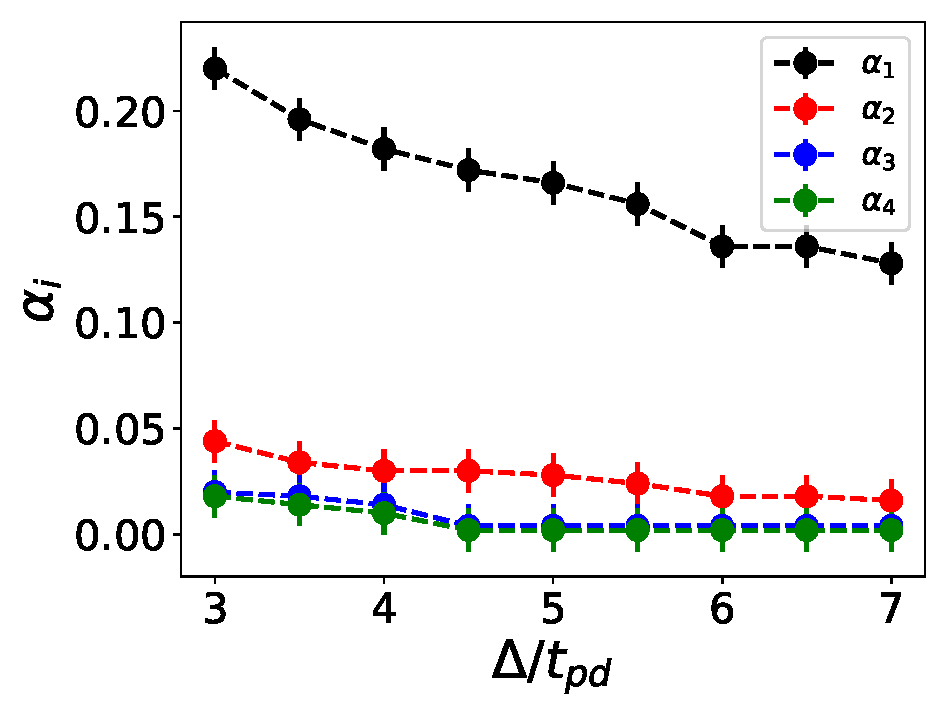
\includegraphics[width=0.49\linewidth]{./Figures/Hyb_vs_ep_Ud_8.pdf}
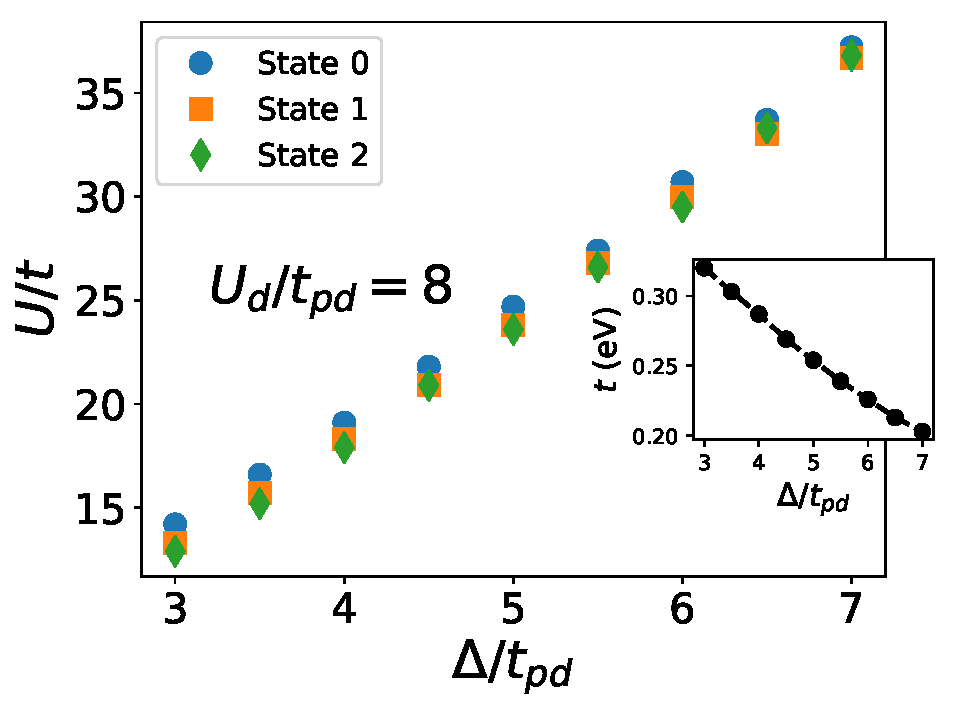
\includegraphics[width=0.49\linewidth]{./Figures/U_and_hopping_combined_vs_ep_Ud_8.pdf}
\caption{(Left) Optimized values of parameters entering the transformation matrix 
($\alpha_1$ through $\alpha_4$) and (Right) Effective 1-band Hubbard $U/t$ and hopping $t$ (inset) 
versus $\Delta/t_{pd}$ for fixed $U_{d}/t_{pd}=8$}
\label{fig:hamfitepdvary} 
\end{figure}	

\begin{figure}[]
\centering
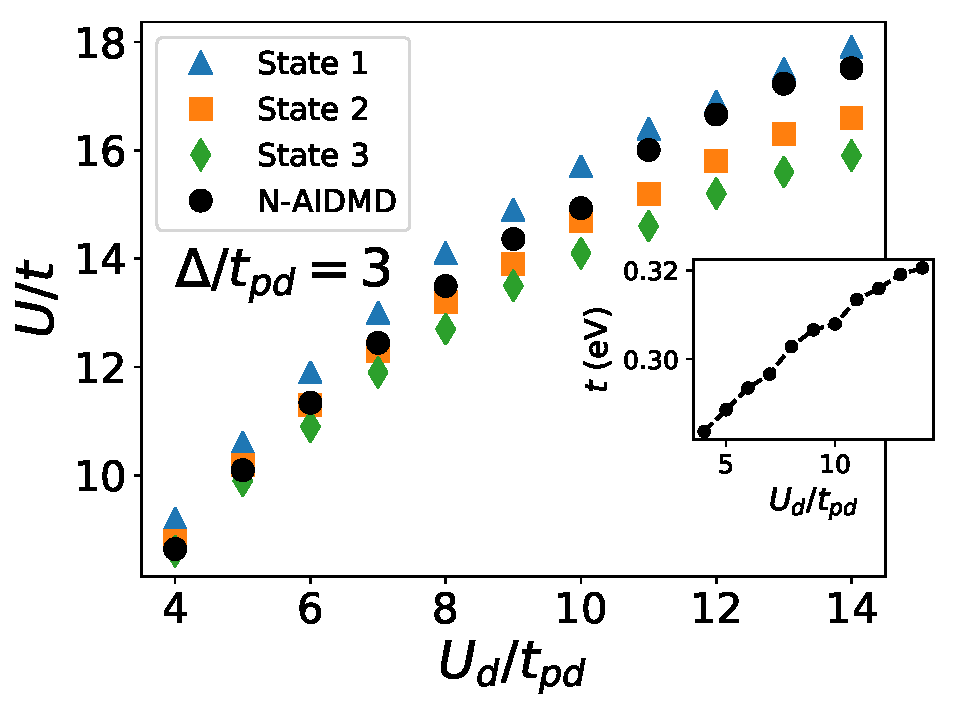
\includegraphics[width=0.48\linewidth]{./Figures/U_and_hopping_combined_vs_Ud_ep_3.pdf}
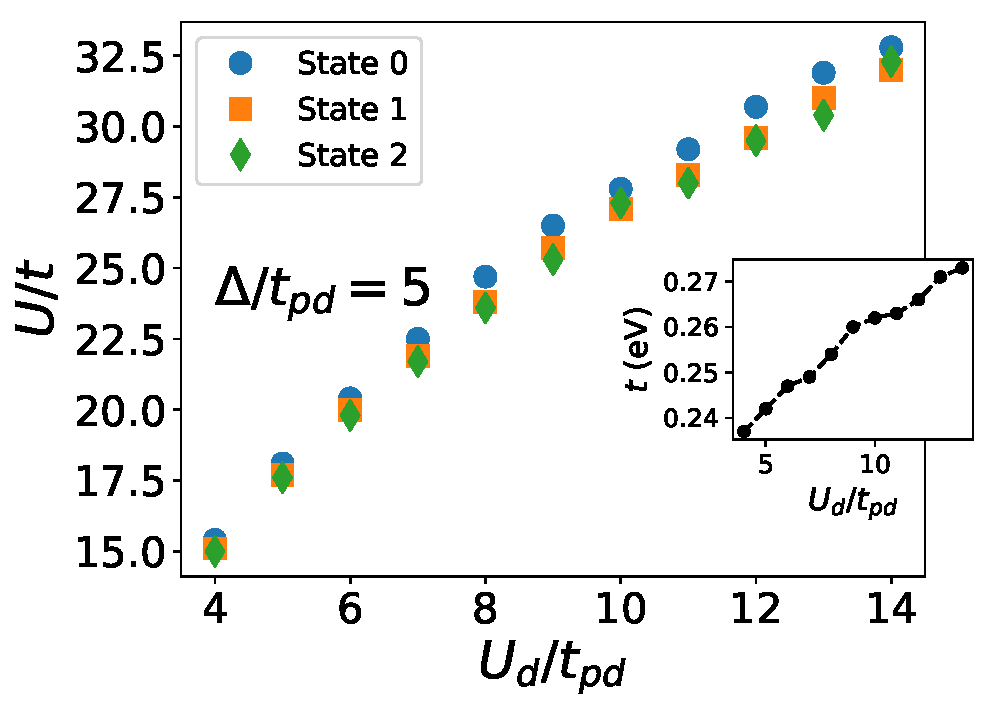
\includegraphics[width=0.50\linewidth]{./Figures/U_and_hopping_combined_vs_Ud_ep_5.pdf}
%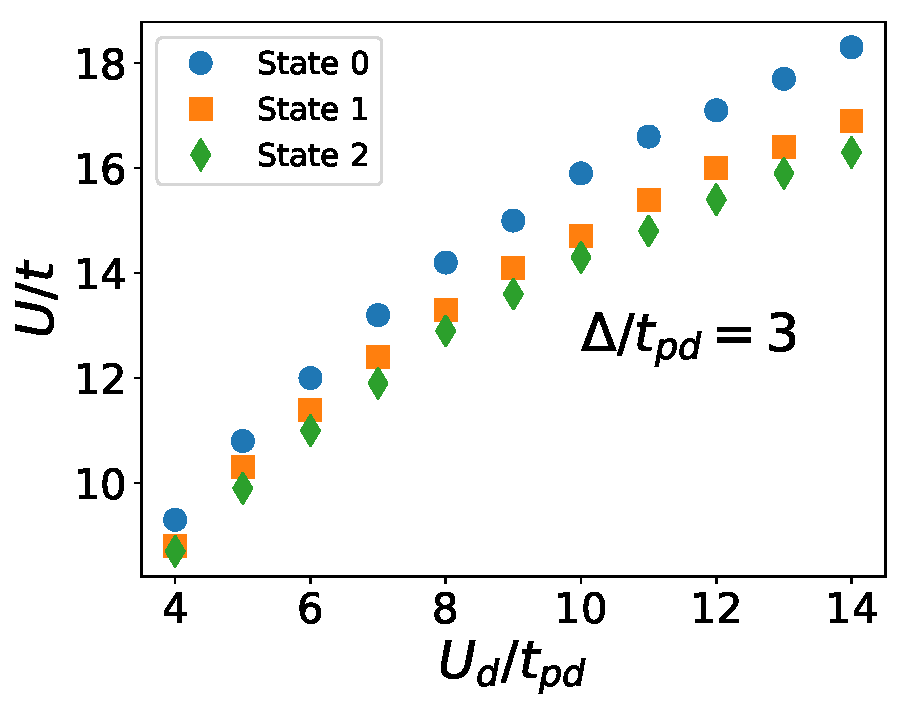
\includegraphics[width=0.49\linewidth]{./Figures/downfolded_U_ep_3.pdf}
%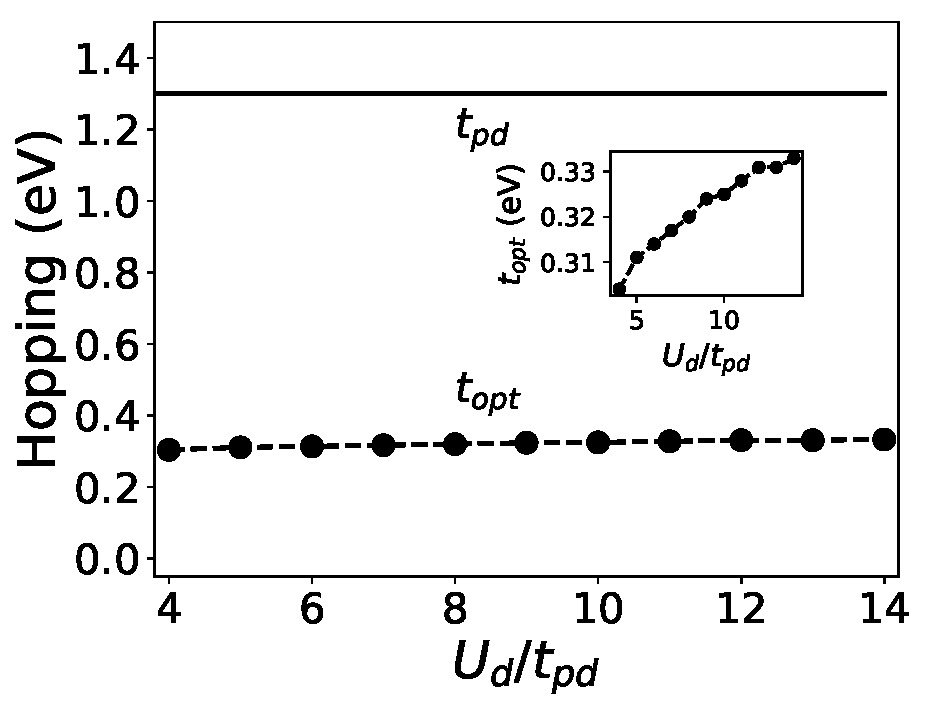
\includegraphics[width=0.49\linewidth]{./Figures/Hopping_vs_U_ep_3.pdf}
%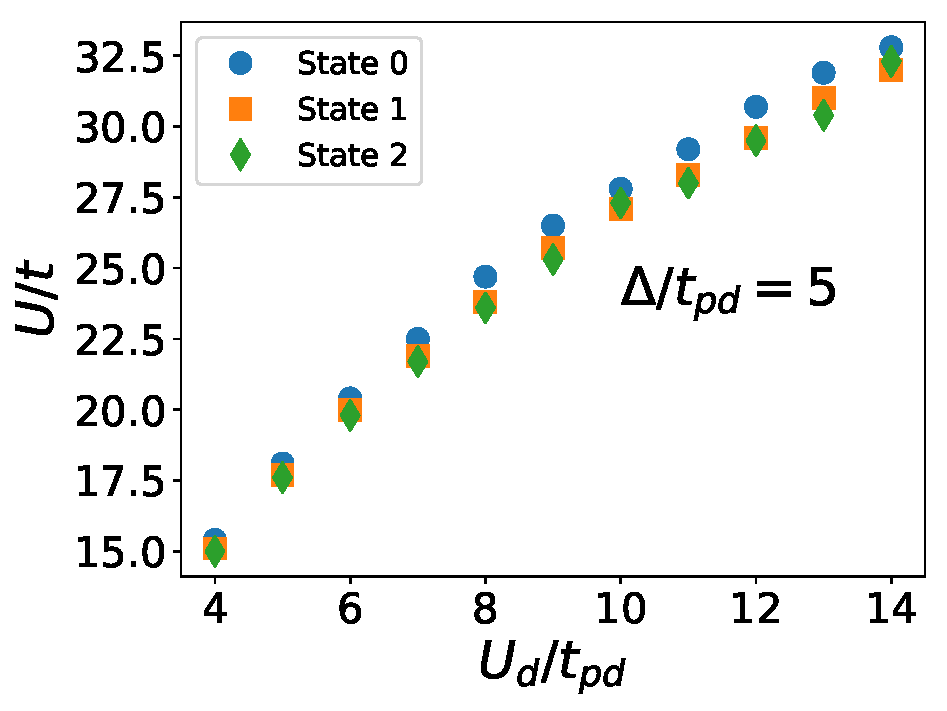
\includegraphics[width=0.49\linewidth]{./Figures/downfolded_U_ep_5.pdf}
%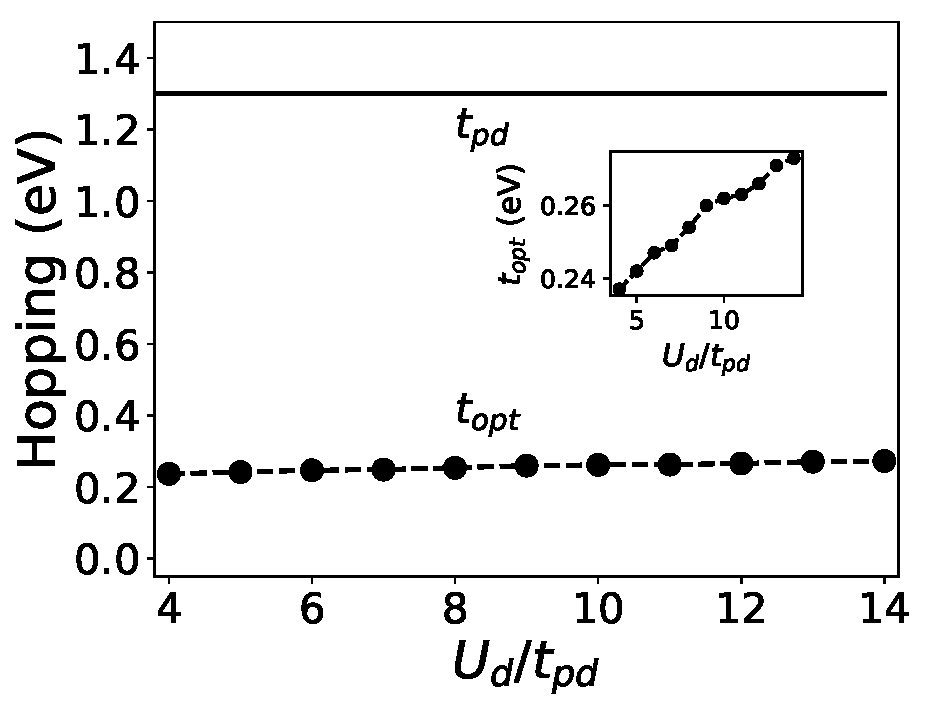
\includegraphics[width=0.49\linewidth]{./Figures/Hopping_vs_U_ep_5.pdf}
\caption{Downfolded values of the effective 1-band Hubbard $U/t$ and $t$ (inset) 
vs $U_d/t_{pd}$ for two representative values of $\Delta/t_{pd}$}
\label{fig:hamfitUdvary} 
\end{figure}	
 
Fig.~\ref{fig:hamfitepdvary} shows our results for the optimal 
transformation parameters ($\alpha$'s), $t$ and $U/t$ as a function of $\Delta/t_{pd}$
keeping $U_d/t_{pd}=8$ fixed. $\alpha_1$, which is the primary parameter that mixes (hybridizes) 
the copper and oxygen orbitals, \textit{decreases} as $\Delta/t_{pd}$ is increased. 
This is physically reasonable since an increasing difference in the single particle energies of the copper and oxygen orbitals 
means that it is even more energetically unfavorable to occupy the oxygen orbitals. 
Correspondingly the effective hopping between $\tilde{d}$ in the 
1-band model reduces and the effective $U/t$ increases. 

Next, in Fig.~\ref{fig:hamfitUdvary} we consider analogous results keeping $\Delta/t_{pd}$ fixed to two representative values, 
and varying $U_d/t_{pd}$. In both cases, $U/t$ increases dramatically with $U_d/t_{pd}$, but $t$ 
increases marginally little (similar results are seen for the dominant 
hybridization parameter $\alpha_1$). Also, the different estimates of $U/t$ are closer to each other 
for the case of larger $\Delta$ indicating the increased effectiveness of the 1-band model 
in the limit of large $\Delta$. 

A primary quality check for the model is its ability to reproduce the low energy spectrum. 
Fig.~\ref{fig:energyfit} shows the comparison of the 1-band vs 3-band model energy gaps 
(here only comprising of $6$ states). In all cases, the fit is reasonably good; 
the best fits seen at larger $U_d$ and larger $\Delta$ consistent with our expectations 
from the previous plots. We re-emphasize that once the density matrices were transformed 
only one parameter ($t$) was fit to match five energy gaps between the two models; this indicates 
it is thus an indicator of the success of the downfolding (rather than a result of overfitting). 

\begin{figure}[]
\centering
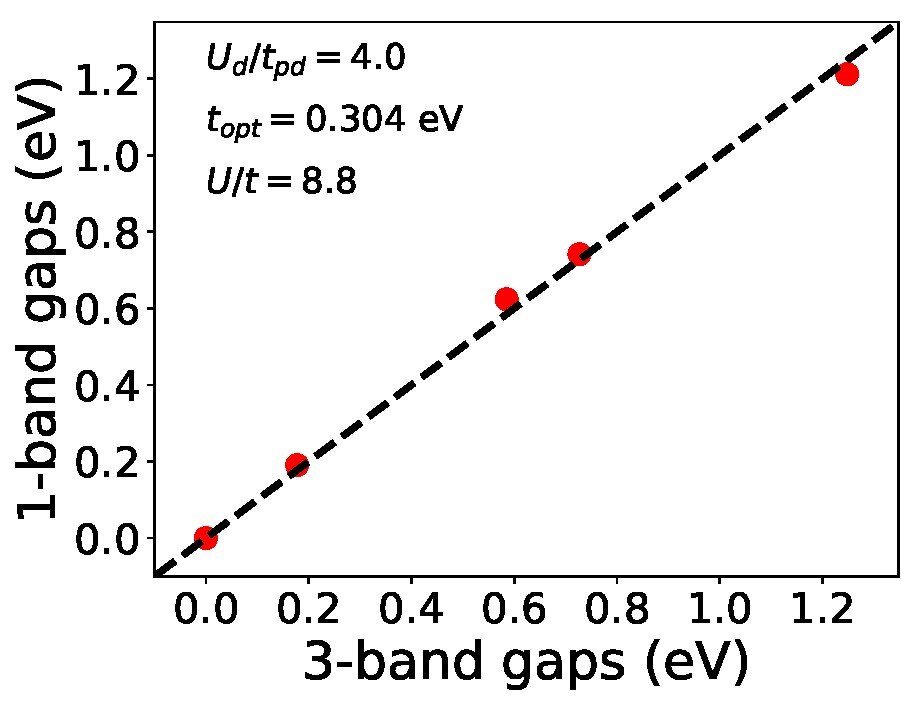
\includegraphics[width=0.325\linewidth]{./Figures/Gap_1_band_3_band_ep_3_number_5.pdf}
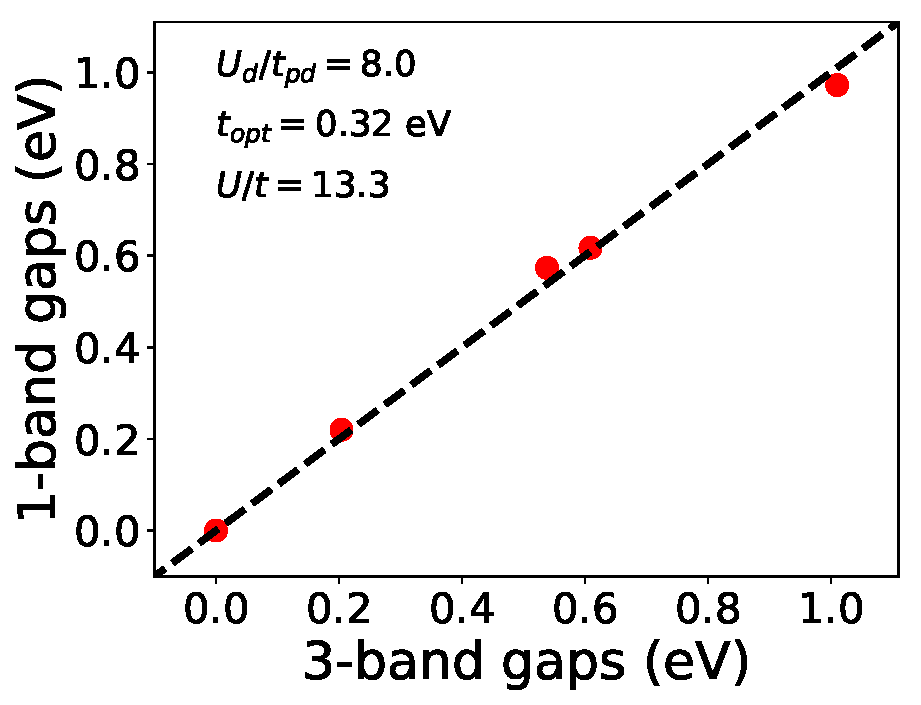
\includegraphics[width=0.325\linewidth]{./Figures/Gap_1_band_3_band_ep_3_number_9.pdf}
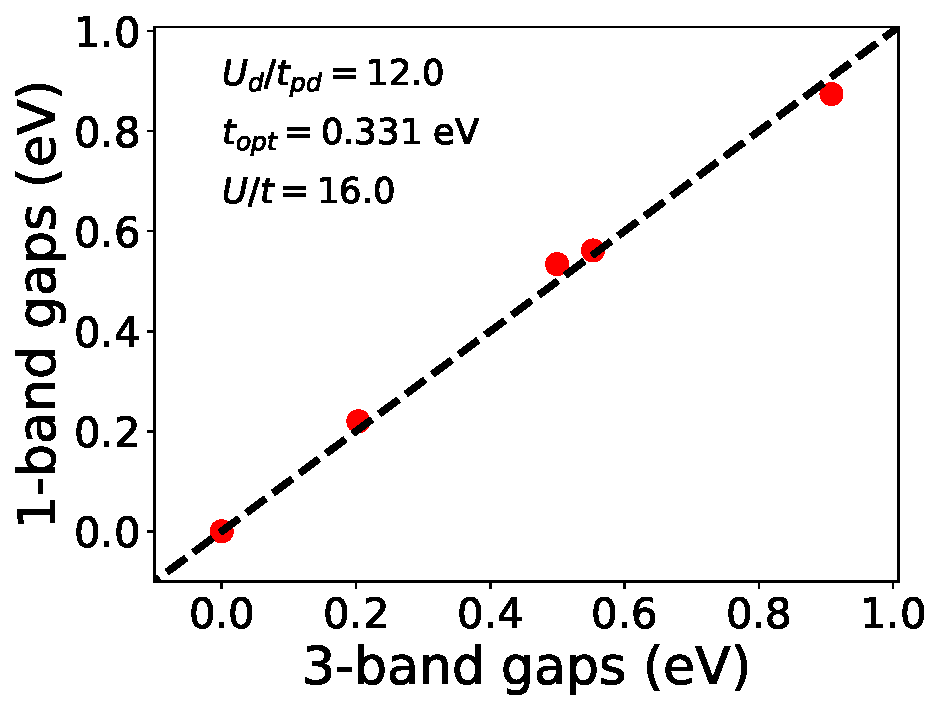
\includegraphics[width=0.325\linewidth]{./Figures/Gap_1_band_3_band_ep_3_number_2.pdf}
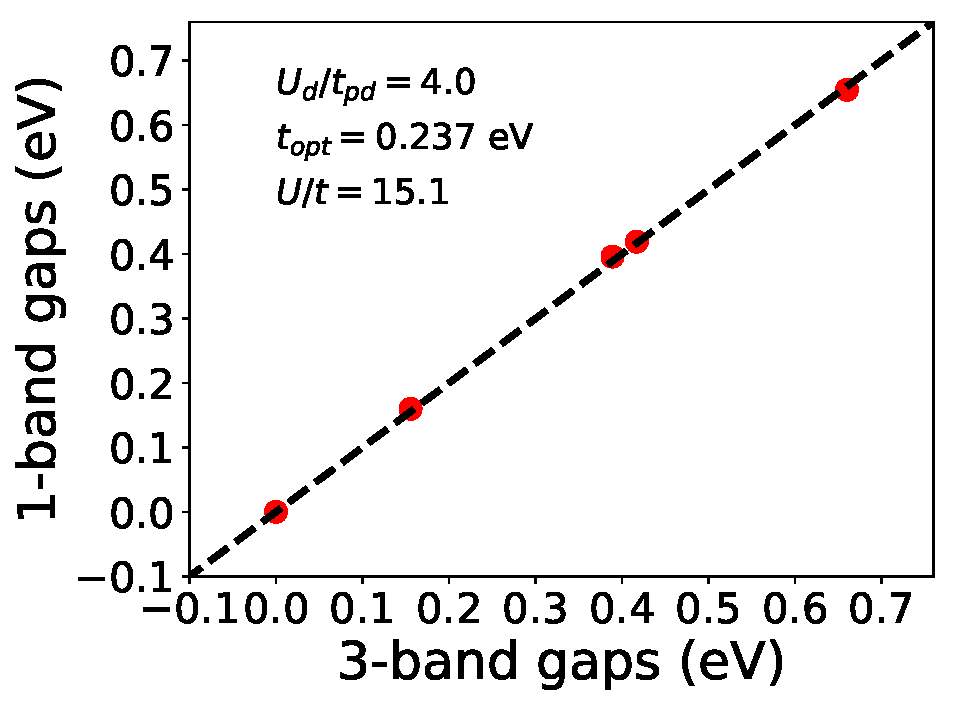
\includegraphics[width=0.325\linewidth]{./Figures/Gap_1_band_3_band_ep_5_number_5.pdf}
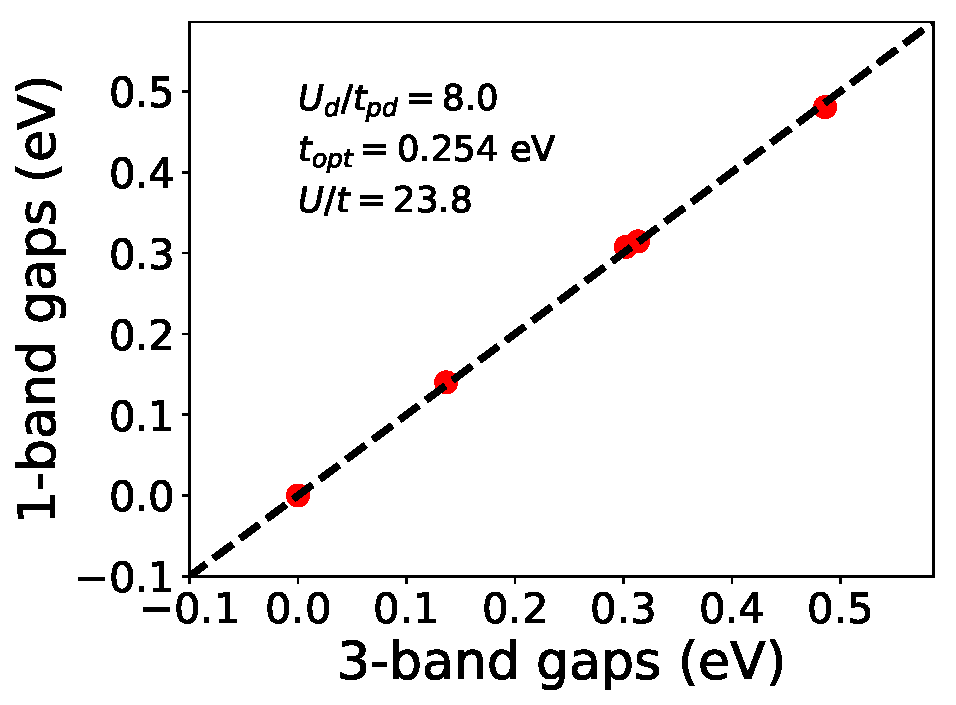
\includegraphics[width=0.325\linewidth]{./Figures/Gap_1_band_3_band_ep_5_number_9.pdf}
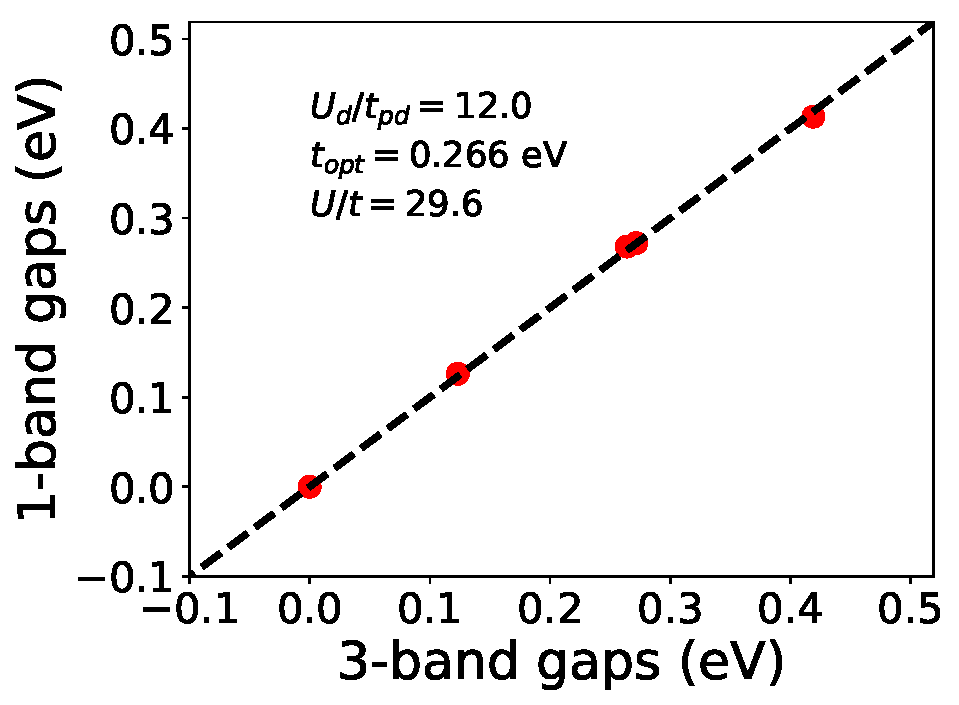
\includegraphics[width=0.325\linewidth]{./Figures/Gap_1_band_3_band_ep_5_number_2.pdf}
\caption{Comparison for energy gaps between the 3-band and 1-band Hubbard models 
using the optimized values of $U/t$ and $t$, for different $U_{d}/t_{pd}$ for $\Delta/t_{pd}=3$ (top row) 
and $\Delta/t_{pd}=5$ (bottom row)}
\label{fig:energyfit} 
\end{figure}	

\HJC {Predictivity} Ultimately, the whole reason for downfolding is to reduce the effective Hilbert space. 
Finally, we show that the obtained parameters are ....

